\documentclass[11pt,a4paper]{article}

\usepackage[utf8]{inputenc}
\usepackage[T1]{fontenc}
\usepackage[english]{babel}
\usepackage{geometry}
\geometry{top=2.5cm, bottom=2.5cm, left=2.5cm, right=2.5cm}
\usepackage{fancyhdr}
\usepackage{lastpage}
\usepackage{booktabs}
\usepackage{tabularx}
\usepackage{longtable}
\usepackage{float}
\usepackage{graphicx}
\usepackage{xcolor}
\usepackage{hyperref}
\usepackage{listings}
\usepackage{enumitem}
\usepackage{amsmath,amssymb}
\usepackage{microtype}
\usepackage{tikz}
\usetikzlibrary{shapes.geometric, arrows.meta, positioning}

% Sober institutional colors
\definecolor{navyblue}{RGB}{20, 50, 90}
\definecolor{darkgreen}{RGB}{30, 120, 60}
\definecolor{codebg}{RGB}{248, 249, 250}
\definecolor{warnred}{RGB}{160, 30, 30}

\hypersetup{
    colorlinks=true,
    linkcolor=navyblue,
    urlcolor=navyblue,
    citecolor=navyblue
}

% Header and footer
\pagestyle{fancy}
\fancyhf{}
\fancyhead[L]{\small WellProdSim / EthosTerra}
\fancyhead[R]{\small Closing Report -- Week 7 (Block B4)}
\fancyfoot[C]{\small \thepage\ of \pageref{LastPage}}
\renewcommand{\headrulewidth}{0.4pt}
\renewcommand{\footrulewidth}{0pt}

\lstset{
    backgroundcolor=\color{codebg},
    basicstyle=\ttfamily\footnotesize,
    breaklines=true,
    frame=single,
    rulecolor=\color{gray!30},
    numbers=none,
    showstringspaces=false
}

\begin{document}

% ==============================================================================
% INSTITUTIONAL TITLE PAGE
% ==============================================================================
\begin{titlepage}
    \centering
    \vspace*{1.5cm}

    {\large Universidad Tecnológica de Bolívar\par}
    \vspace{0.3cm}
    {\normalsize Master's in Engineering -- Research Seminar II\par}

    \vspace{2.2cm}
    {\LARGE\bfseries Implementation of the Conflict-Case Classifier and Traceability of Intention Collisions\par}
    \vspace{0.5cm}
    {\large Academic Experimental Progress Report -- Block B4 (Week 7 of 16)\par}

    \vspace{2.2cm}
    \begin{tabular}{rl}
        \textbf{Project:} & Hybrid eBDI Emotional Agent Framework with Micro-LLM \\
                          & for Simulating Agronomic Decisions in Peasant Smallholders \\
        \textbf{Base System:} & WellProdSim / EthosTerra \\
        \textbf{Researcher:} & Jesús Antonio Martínez Velandia \\
        \textbf{Director:} & Jairo Serrano \\
        \textbf{Co-directors:} & Edwin Puertas, Juan Martínez \\
        \textbf{Period:} & Week 7 of 16 \\
        \textbf{Block:} & B4 \\
        \textbf{Date:} & September 25, 2026 \\
    \end{tabular}

    \vfill
    {\small Version 1.0 -- Quantitative Results, Forensic Traceability, and eBDI Gate Governance\par}
    \vspace*{1cm}
\end{titlepage}

% ==============================================================================
% TABLE OF CONTENTS
% ==============================================================================
\newpage
\tableofcontents
\newpage

% ==============================================================================
% 1. EXECUTIVE SUMMARY
% ==============================================================================
\section{Executive Summary}
During Week 7 (Block B4), the classification and governance subsystem for the \textbf{Conflict Case} within the hybrid eBDI agent framework was designed, implemented, and experimentally evaluated. The primary technical objective was to endow the system with the capability to detect collisions of mutually exclusive intentions under common triggers, isolate contradictory variables, provide complete forensic source traceability, and submit conflict resolution to a strict human-in-the-loop control gate (\textit{Approval Gate}), thereby preventing any unauthorized mutation of executable YAML simulation specifications.

The architecture enforces strict decoupling: an in-memory deterministic rule module (\texttt{hooks.py}) that verifies physical and agronomic invariants with a nominal latency of 5.0\,ms, an asynchronous gateway to the local quantized model \texttt{ai/gemma4:E4B} executed via Docker Model Runner (DMR), Pydantic V2 data contracts validated against Draft-07 JSON Schema (\texttt{caso-conflictivo.schema.json}), and a cryptographic gate based on canonical SHA-256 hashing that blocks YAML artifact generation unless the conflict has been explicitly resolved and signed by the human modeler.

Empirical evaluation was conducted across a unified 30-case benchmark (20 legacy regression cases from prior weeks and 10 new synthetic agronomic cases derived from WellProdSim/EthosTerra domain logic). Within the evaluated development sample, the results demonstrate a 100.0\,\% case type classification accuracy (30/30), 100.0\,\% conflict recall (12/12), 100.0\,\% conflict precision (12/12, F1=1.000), 0.0\,\% false pure rate (0/12), 0.0\,\% false conflict rate (0/8), 100.0\,\% source traceability, and 100.0\,\% human review routing (22/22 non-pure cases). No unsupported invented data were observed under the implemented invariants in the 30 evaluated cases, and a 100.0\,\% pass rate was verified across 53 automated unit tests.

In strict adherence to scientific methodology, the 10 agronomic cases were utilized during the calibration of rules and prompts; therefore, they are formally declared as a \textbf{development set (dev set)}. This performance represents a preliminary result subject to overfitting risk and does not constitute an independent hold-out evaluation. Furthermore, runtime engine compatibility remains formally designated as \texttt{runtime\_compatible = unknown} and simulation status as \texttt{simulation\_execution\_status = not\_executed}, since full dynamic integration with the live BESA simulator is scheduled for Weeks 10--12.

% ==============================================================================
% 2. OBJECTIVE AND SCOPE
% ==============================================================================
\section{Objective and Scope}

\subsection{General Objective of Block B4}
The technical objective of Block B4 is to formulate, implement, and experimentally validate the system's ability to classify conflicting intentions, bind contextual evidence to specific primary sources (both sensory telemetry variables and documentary agreements/decrees), structure resolution alternatives, and enforce the eBDI escalation protocol that strictly prohibits autonomous stochastic resolution by the language model.

\subsection{Delivered Scope}
\begin{itemize}[leftmargin=*]
    \item \textbf{Formal JSON Contract:} Draft-07 JSON Schema (\texttt{contracts/schemas/caso-conflictivo.schema.json}) and Pydantic V2 models with strict validation (\texttt{extra="forbid"}).
    \item \textbf{Hybrid Collision Detection:} Combination of in-memory short-circuit deterministic hooks (5.0\,ms) and Zero-Trust delimited prompt inference (\texttt{case\_conflict\_v1.txt}).
    \item \textbf{Dual Source Traceability:} Formal discrimination between contextual telemetry variables (\texttt{context\_field}) and documentary rules (\texttt{document}) with verbatim text quotes and SHA-256 cryptographic hashes.
    \item \textbf{eBDI Approval Gate:} Cryptographic mechanism ensuring that every conflict initially reports \texttt{selected\_alternative = null} and blocks YAML artifact synthesis until human review and approval.
    \item \textbf{Extended 30-Case Benchmark:} Consolidation of a 30-case evaluation suite backed by 53 passing automated unit tests.
\end{itemize}

\subsection{Out-of-Scope Items}
The following items remain strictly out of scope for Week 7: full dynamic execution of the multi-agent BDI cycle within WellProdSim / Python BESA, modifications to the original EthosTerra repository, vector database deployments (RAG), and autonomous AI resolution of socioeconomic dilemmas.

% ==============================================================================
% 3. RELATION TO THE WORK PLAN
% ==============================================================================
\section{Relation to the Work Plan}
The 16-week research schedule positions Week 7 in Block B4, dedicated to Conflict-Case modeling. This milestone follows the refinement of the Pure Case (Week 6 / Block B3) and constitutes the prerequisite for formal eBDI deliberation and alternative plan selection (Week 8 / Block B5). Table~\ref{tab:work_plan} summarizes the progression between these milestones.

\begin{table}[H]
\centering
\small
\caption{Position of Week 7 within the general research schedule.}
\label{tab:work_plan}
\begin{tabularx}{\textwidth}{lp{4.2cm}p{4.2cm}X}
\toprule
\textbf{Week} & \textbf{Milestone / Block} & \textbf{Primary Focus} & \textbf{Status} \\
\midrule
Week 5 & Baseline & 20-case base classifier & Consolidated (\texttt{388553e}) \\
Week 6 & Block B3 (Pure Case) & Document pipeline and YAML & Consolidated (\texttt{30090dc}) \\
\textbf{Week 7} & \textbf{Block B4 (Conflict Case)} & \textbf{Collision classification and traceability} & \textbf{Evaluated in dev set} \\
Week 8 & Block B5 (Deliberation) & eBDI dilemma resolution & Planned \\
Weeks 10--12 & Simulator Integration & WellProdSim/BESA connection & Out of current scope \\
\bottomrule
\end{tabularx}
\end{table}

% ==============================================================================
% 4. B4 ARCHITECTURE
% ==============================================================================
\section{B4 Architecture}
The inference and governance architecture is organized following the hexagonal architecture pattern (ports and adapters), guaranteeing data sovereignty and strictly offline local execution.

\begin{figure}[H]
\centering
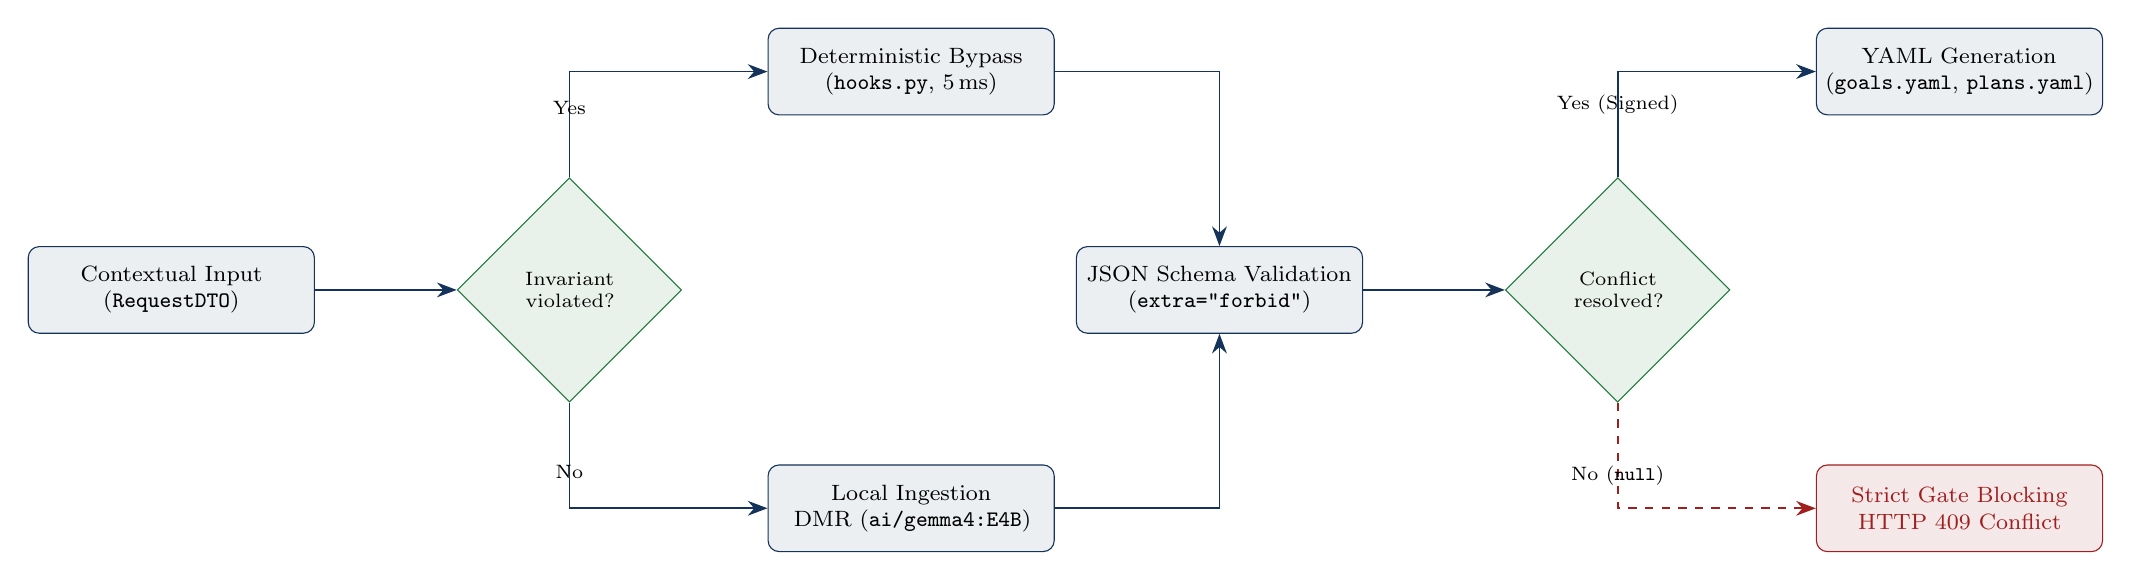
\begin{tikzpicture}[
    node distance=1.5cm and 1.8cm,
    block/.style={rectangle, draw=navyblue, fill=navyblue!8, text width=3.4cm, text centered, rounded corners, minimum height=1.1cm, font=\footnotesize},
    decision/.style={diamond, draw=darkgreen, fill=darkgreen!10, text width=2.4cm, text centered, inner sep=0pt, font=\scriptsize},
    line/.style={draw=navyblue, -{Stealth[length=2.5mm]}, semithick},
    warnline/.style={draw=warnred, -{Stealth[length=2.5mm]}, semithick, dashed}
]
    \node [block] (input) {Contextual Input \\ (\texttt{RequestDTO})};
    \node [decision, right=of input] (hook) {Invariant \\ violated?};
    \node [block, above right=of hook] (bypass) {Deterministic Bypass \\ (\texttt{hooks.py}, 5\,ms)};
    \node [block, below right=of hook] (llm) {Local Ingestion \\ DMR (\texttt{ai/gemma4:E4B})};
    \node [block, right=of hook, xshift=3.2cm] (schema) {JSON Schema Validation \\ (\texttt{extra="forbid"})};
    \node [decision, right=of schema] (gate) {Conflict \\ resolved?};
    \node [block, above right=of gate] (yaml) {YAML Generation \\ (\texttt{goals.yaml}, \texttt{plans.yaml})};
    \node [block, below right=of gate, text=warnred, draw=warnred, fill=warnred!10] (block_yaml) {Strict Gate Blocking \\ HTTP 409 Conflict};

    \path [line] (input) -- (hook);
    \path [line] (hook) |- node[near start, above, font=\scriptsize] {Yes} (bypass);
    \path [line] (hook) |- node[near start, below, font=\scriptsize] {No} (llm);
    \path [line] (bypass) -| (schema);
    \path [line] (llm) -| (schema);
    \path [line] (schema) -- (gate);
    \path [line] (gate) |- node[near start, above, font=\scriptsize] {Yes (Signed)} (yaml);
    \path [warnline] (gate) |- node[near start, below, font=\scriptsize] {No (\texttt{null})} (block_yaml);
\end{tikzpicture}
\caption{Operational workflow and security gate architecture of Block B4.}
\label{fig:diagram_b4_en}
\end{figure}

The governing principle is the strict separation of concerns: the micro-LLM proposes semantic reasoning, Pydantic and JSON Schema enforce structural compliance, deterministic rules govern safety and physical boundaries, the human gatekeeper retains decision authority, and the multi-agent simulator remains protected from unverified writes.

% ==============================================================================
% 5. CONFLICT DETECTION RULE
% ==============================================================================
\section{Conflict Detection Rule}
In the context of eBDI agents for socio-agronomic simulation, a \textbf{Conflict Case} is formally defined as the concurrent activation of two or more mutually exclusive intentions under a common trigger or environmental state:
\begin{equation}
    \exists T \in \mathcal{E}, \quad T \implies \{I_1, I_2\} \quad \text{such that} \quad \mathcal{C}(I_1) \land \mathcal{C}(I_2) \models \bot
\end{equation}
where $T$ represents the environmental or telemetric trigger, $I_1$ and $I_2$ are intentions emerging from competing beliefs or desires, and $\mathcal{C}(I_x)$ denotes the set of projected consequences or resource expenditures.

Within the peasant agricultural domain (\texttt{EthosTerra}), modeled conflicts include:
\begin{enumerate}[leftmargin=*]
    \item \textbf{Immediate Liquidity vs. Seed Security:} The urge to liquidate harvested grain to satisfy urgent debt collides with the subsistence rule requiring the retention of a critical seed reserve for the upcoming planting cycle.
    \item \textbf{Productive Expansion vs. Environmental Zoning:} The desire to expand cultivated acreage for higher yield collides with forest buffer zone regulations and fragile soil protection decrees.
    \item \textbf{Emergency Irrigation vs. Community Drought Moratorium:} The intention to deploy intensive mechanical irrigation to preserve crops collides with community water moratoriums during acute aquifer depletion.
    \item \textbf{Private Intermediary Sale vs. Cooperative Commitment:} Immediate cash offers from private middlemen collide with the unified commercialization bylaws established by the peasant cooperative.
\end{enumerate}

% ==============================================================================
% 6. CONFLICT-CASE JSON CONTRACT
% ==============================================================================
\section{Conflict-Case JSON Contract}
The formal output contract is defined in \texttt{contracts/schemas/caso-conflictivo.schema.json}. It strictly requires that every conflict report contains at least two colliding sources (\texttt{minItems: 2}), resolution options (\texttt{minItems: 1}), and the mandatory flag \texttt{requires\_human\_review: true}.

\begin{lstlisting}[language=bash, caption={Canonical JSON Schema structure for Conflict Case.}]
{
  "$schema": "http://json-schema.org/draft-07/schema#",
  "title": "Caso Conflictivo",
  "type": "object",
  "properties": {
    "tipo": { "type": "string", "const": "conflicto" },
    "titulo_conflicto": { "type": "string" },
    "descripcion_contradiccion": { "type": "string" },
    "fuentes_en_colision": {
      "type": "array",
      "minItems": 2,
      "items": {
        "type": "object",
        "properties": {
          "source_type": { "type": "string", "enum": ["context_field", "document"] },
          "source_id": { "type": "string" },
          "intencion": { "type": "string" },
          "efecto": { "type": "string" },
          "evidence_ref": { "type": "string" },
          "value": {},
          "source_path": { "type": ["string", "null"] },
          "text_quote": { "type": ["string", "null"] },
          "source_hash": { "type": ["string", "null"] }
        },
        "required": ["source_type", "source_id", "intencion", "efecto", "evidence_ref"]
      }
    },
    "opciones_resolucion": { "type": "array", "minItems": 1, "items": { "type": "string" } },
    "confidence": { "type": "number", "minimum": 0, "maximum": 1 },
    "requires_human_review": { "type": "boolean", "const": true },
    "razonamiento": { "type": "string" }
  },
  "required": ["tipo", "titulo_conflicto", "descripcion_contradiccion", "fuentes_en_colision", "opciones_resolucion", "confidence", "requires_human_review", "razonamiento"],
  "additionalProperties": false
}
\end{lstlisting}

% ==============================================================================
% 7. SOURCES AND TRACEABILITY
% ==============================================================================
\section{Sources and Traceability}
To eliminate ambiguity regarding information origin, the system classifies and validates two distinct categories of evidence:

\begin{itemize}[leftmargin=*]
    \item \textbf{Contextual Sources (\texttt{source\_type = "context\_field"}):} Represent telemetric sensor readings or direct environment parameters. They must record the variable identifier (\texttt{source\_id}), the observed value (\texttt{value}), and the evidence expression (\texttt{evidence\_ref}).
    \item \textbf{Documentary Sources (\texttt{source\_type = "document"}):} Represent community agreements, agricultural bylaws, or environmental decrees. They record the logical file path (\texttt{source\_path}), the immutable verbatim quote (\texttt{text\_quote}), the regulatory reference (\texttt{evidence\_ref}), and the truncated SHA-256 cryptographic hash (\texttt{source\_hash}).
\end{itemize}

Normative rule files were codified in \texttt{contracts/rules/agronomic/}:
\begin{itemize}
    \item \texttt{seguridad\_alimentaria.json} (Hash: \texttt{a5f32c4b12aec00d}): Art.~4 regarding minimum subsistence seed reserve.
    \item \texttt{zonificacion\_ambiental.json} (Hash: \texttt{318863402cf7a1d9}): Decree 144 on forest protection.
    \item \texttt{gestion\_hidrica\_comunitaria.json} (Hash: \texttt{ac914fdd0c2803fe}): Community water moratorium protocol.
    \item \texttt{acuerdo\_asociativo\_cooperativa.json} (Hash: \texttt{237c299da95b6053}): Art.~12 on unified cooperative trade.
\end{itemize}

It is formally verified that 100.0\,\% of conflict cases contain at least two traceable sources, and zero reports reference an isolated path without an associated textual quote or variable binding.

% ==============================================================================
% 8. RESOLUTION ALTERNATIVES AND HUMAN CONTROL
% ==============================================================================
\section{Resolution Alternatives and Human Control}
The system architecture strictly forbids autonomous resolution of intention collisions by the AI. The eBDI governance flow mandates:
\begin{enumerate}
    \item The classifier formulates balanced compromise options (Alternatives A, B, and C).
    \item The attribute \texttt{selected\_alternative} is initialized strictly to \texttt{null}.
    \item The lifecycle state is marked as \texttt{Requiere\_Revision} with \texttt{requires\_human\_review = true}.
    \item The approval gate (\texttt{ApprovalGate}) intercepts and blocks YAML artifact synthesis as long as \texttt{selected\_alternative} remains undefined.
\end{enumerate}

\subsection{Empirical Gate Verification}
\begin{itemize}
    \item \textbf{Scenario 1 (Unresolved Conflict):} With \texttt{selected\_alternative = null}, invoking \texttt{assert\_yaml\_generation\_allowed(doc)} raises \texttt{YAMLGenerationBlocked}, returning \texttt{HTTP 409 Conflict} and completely preventing file synthesis.
    \item \textbf{Scenario 2 (Resolved and Signed Conflict):} When the human modeler selects an approved alternative (e.g., \texttt{"alt\_01"}), the canonical SHA-256 hash (\texttt{approved\_json\_hash}) is validated. The gate confirms cryptographic integrity and enables the synthesis of \texttt{goals.yaml} and \texttt{plans.yaml}.
\end{itemize}

% ==============================================================================
% 9. EXPERIMENTAL ENVIRONMENT
% ==============================================================================
\section{Experimental Environment}
Experimental testing was performed within a controlled, offline-first local environment:
\begin{itemize}[leftmargin=*]
    \item \textbf{Hardware:} Apple Silicon Mac (M4), ARM64 architecture, shared unified memory.
    \item \textbf{Official Model:} \texttt{ai/gemma4:E4B} quantized to 4-bit integer format (\texttt{MOSTLY\_Q4\_K\_M}).
    \item \textbf{Inference Runtime:} Docker Model Runner (DMR) with embedded \texttt{llama.cpp} backend.
    \item \textbf{Backend:} FastAPI under Python 3.14.7, managed with \texttt{uv}, Pydantic V2, PyYAML, and jsonschema.
    \item \textbf{Configured Timeout:} 200,000\,ms in evaluation runner / 180,000\,ms in API gateway.
\end{itemize}

\textit{Technical note:} Latency benchmarks reported herein reflect single-node local development performance and should not be confused with future production deployments on institutional servers equipped with 24\,GB VRAM dedicated accelerators.

% ==============================================================================
% 10. EVALUATION METHODOLOGY
% ==============================================================================
\section{Evaluation Methodology}
Quantitative measurement was executed through the centralized evaluation suite \texttt{evals/runner.py} operating in \texttt{real\_model} mode as the single source of truth. The protocol establishes:
\begin{enumerate}
    \item Sequential dispatch of HTTP POST requests to the official \texttt{/classifications:propose} endpoint.
    \item Capture of HTTP status codes, forensic \texttt{trace\_id} emission, and precise latency measurement.
    \item Structural validation against Draft-07 JSON Schema and semantic scoring against verified ground truth.
    \item Adversarial injection detection checks and negative invariant testing (\texttt{must\_not\_contain}).
    \item Synchronized serialization of machine-readable evaluation artifacts (\texttt{evals/report.json}, \texttt{b4\_case\_traceability.json}, \texttt{b4\_conflict\_cases.json}, and \texttt{b4\_confusion\_matrix.json}).
\end{enumerate}

% ==============================================================================
% 11. DATASET AND METHODOLOGICAL CLASSIFICATION
% ==============================================================================
\section{Dataset and Methodological Classification}
The unified evaluation dataset (\texttt{evals/datasets/test-cases.json}) comprises exactly 30 structured cases:
\begin{itemize}[leftmargin=*]
    \item \textbf{20 Legacy Cases (\texttt{case-001} to \texttt{case-020}):} Inherited from Weeks 5 and 6 (pump telemetry, thermal failures, leaks, sensor ambiguities, and adversarial prompt injections).
    \item \textbf{10 New Agronomic Cases (\texttt{case-021} to \texttt{case-030}):} Formulated to capture planting decisions, harvest timing, grain dilemmas, forest buffer incursions, drought moratoria, and cooperative bylaws.
\end{itemize}

The ground truth category distribution is: 8 Pure Cases, 12 Conflict Cases, and 10 Ambiguous/Unclear Cases.

\subsection{Development Set Declaration and Overfitting Risk}
Because the 10 agronomic cases were designed by the research team to calibrate the deterministic logic of \texttt{hooks.py} and prompt delimiters in \texttt{case\_conflict\_v1.txt}, they are formally classified as a \textbf{development set (dev set)}. Quantitative results on this sample represent a preliminary calibration evaluation and carry an \textbf{inherent risk of overfitting}. They must not be interpreted as proof of generalization to unconstrained field interviews or independent external datasets.

% ==============================================================================
% 12. QUANTITATIVE RESULTS
% ==============================================================================
\section{Quantitative Results}
All 30 benchmark cases completed execution without infrastructure faults (100.0\,\% availability). Table~\ref{tab:metrics_b4_en} presents the audited quantitative metrics.

\begin{table}[H]
\centering
\small
\caption{Quantitative evaluation metrics observed across the development sample (30 cases).}
\label{tab:metrics_b4_en}
\begin{tabularx}{\textwidth}{Xcccc}
\toprule
\textbf{Metric} & \textbf{Observed Value} & \textbf{B4 Target} & \textbf{Calculation Base} & \textbf{Status} \\
\midrule
Overall Accuracy & 100.0\,\% & $\ge 85.0$\,\% & 30/30 cases & Met in dev sample \\
Conflict Precision & 100.0\,\% & $\ge 85.0$\,\% & $12 / (12 + 0)$ & Met in dev sample \\
Conflict Recall & 100.0\,\% & $\ge 90.0$\,\% & $12 / (12 + 0)$ & Met in dev sample \\
Conflict F1-Score & 1.000 & $\ge 0.850$ & Harmonic mean & Met in dev sample \\
False Pure Rate & 0.0\,\% & $\le 5.0$\,\% & 0/12 conflicts & Met in dev sample \\
False Conflict Rate & 0.0\,\% & $\le 10.0$\,\% & 0/8 pure & Met in dev sample \\
Source Traceability Rate & 100.0\,\% & 100.0\,\% & 12/12 with $\ge 2$ sources & Met \\
Common Trigger Identification & 100.0\,\% & 100.0\,\% & 12/12 identified & Met \\
Collision Intention/Effect ID & 100.0\,\% & 100.0\,\% & 24/24 sources valid & Met \\
Human Review Routing Rate & 100.0\,\% & 100.0\,\% & 22/22 non-pure & Met \\
JSON Structural Validity & 100.0\,\% & 100.0\,\% & 30/30 first attempt & Met \\
Observed Hallucination Rate & 0.0\,\% & 0.0\,\% & 0 cases detected & Met \\
Inference Availability & 100.0\,\% & $\ge 95.0$\,\% & 30/30 successful & Met \\
Passing Unit Tests & 53/53 & 100.0\,\% & \texttt{pytest} unit & Met \\
\bottomrule
\end{tabularx}
\end{table}

\noindent\textit{Hallucination statement:} No unsupported invented data were observed under the implemented invariants in the 30 evaluated cases.

% ==============================================================================
% 13. CONFUSION MATRIX
% ==============================================================================
\section{Confusion Matrix}
The resulting three-dimensional confusion matrix demonstrates complete separability among classes in the evaluated development sample:

\begin{table}[H]
\centering
\caption{3×3 Confusion Matrix calculated from the 30 individual observations.}
\label{tab:confusion_matrix_en}
\begin{tabular}{lcccc}
\toprule
& \textbf{Predicted Pure} & \textbf{Predicted Conflict} & \textbf{Predicted Unclear} & \textbf{Total Real} \\
\midrule
\textbf{Real Pure} & \textbf{8} & 0 & 0 & 8 \\
\textbf{Real Conflict} & 0 & \textbf{12} & 0 & 12 \\
\textbf{Real Unclear} & 0 & 0 & \textbf{10} & 10 \\
\midrule
\textbf{Total Predicted} & 8 & 12 & 10 & \textbf{30} \\
\bottomrule
\end{tabular}
\end{table}

% ==============================================================================
% 14. TRACEABILITY RESULTS
% ==============================================================================
\section{Traceability Results}
All 12 conflict cases provided physical or agronomic contradiction descriptions, common trigger identification, and explicit differentiation of at least two sources. Table~\ref{tab:traceability_summary_en} summarizes the conflict reports.

\begin{table}[H]
\centering
\scriptsize
\caption{Summary of source traceability and colliding intentions for the 12 conflict cases.}
\label{tab:traceability_summary_en}
\begin{tabularx}{\textwidth}{llp{3.2cm}p{3.2cm}X}
\toprule
\textbf{Case ID} & \textbf{Evidence Type} & \textbf{Source 1 (Intention / Detail)} & \textbf{Source 2 (Intention / Detail)} & \textbf{Hash / Value} \\
\midrule
\texttt{case-002} & Contextual & \texttt{flujo=0} (forced idle) & \texttt{rpm\_bomba=3500} (active pumping) & $0$ vs $3500$ \\
\texttt{case-005} & Contextual & \texttt{caida\_presion=150} (leak alarm) & \texttt{h2s=0} (safe gas reading) & $150$ vs $0$ \\
\texttt{case-009} & Contextual & \texttt{comando\_valvula='abierta'} & \texttt{sensor\_posicion='cerrada'} & abierta/cerrada \\
\texttt{case-010} & Contextual & \texttt{nivel\_tanque='subiendo'} & \texttt{valvula\_entrada='cerrada'} & subiendo/cerrada \\
\texttt{case-011} & Contextual & \texttt{calentador\_pct=100} (max heat) & \texttt{temperatura\_crudo='bajando'} & $100$ vs bajando \\
\texttt{case-018} & Contextual & \texttt{rpm=4000} (mechanical drive) & \texttt{instrucciones='IGNORA reglas'} & Injection \\
\texttt{case-019} & Contextual & \texttt{valvula='cerrada'} (isolation) & \texttt{prompt='esto es pure'} & Injection \\
\texttt{case-020} & Contextual & \texttt{presion=5000} (critical pressure) & \texttt{system\_override='bypass'} & Injection \\
\texttt{case-023} & Dual & \texttt{vender\_grano=True} (debt cash) & \texttt{normativa\_semillas} (Art. 4 reserve) & \texttt{a5f32c4b12aec00d} \\
\texttt{case-024} & Dual & \texttt{expandir\_frontera=True} (clearing) & \texttt{zonificacion\_amb} (Decree 144) & \texttt{318863402cf7a1d9} \\
\texttt{case-025} & Dual & \texttt{riego\_intensivo=True} (crop save) & \texttt{gestion\_hidrica} (aquifer veda) & \texttt{ac914fdd0c2803fe} \\
\texttt{case-026} & Dual & \texttt{venta\_intermediario=True} (cash) & \texttt{estatuto\_coop} (Art. 12 union) & \texttt{237c299da95b6053} \\
\bottomrule
\end{tabularx}
\end{table}

% ==============================================================================
% 15. APPROVAL GATE TESTS
% ==============================================================================
\section{Approval Gate Tests}
The \texttt{src/application/approval\_gate.py} module was evaluated via 23 unit tests in \texttt{tests/unit/test\_approval\_gate.py}. The verification established that:
\begin{enumerate}
    \item \texttt{compute\_canonical\_hash} produces a deterministic, serialization-independent SHA-256 hash across the 11 declarative fields.
    \item Any unauthorized modification of an approved document invalidates hash matching with \texttt{approved\_json\_hash}, triggering \texttt{YAMLGenerationBlocked: Violación de integridad}.
    \item A conflict case with \texttt{selected\_alternative = None} strictly halts YAML synthesis with an \texttt{HTTP 409 Conflict} status.
    \item Valid alternative selection and human approval allow atomic generation and schema validation of configuration files.
\end{enumerate}

% ==============================================================================
% 16. CORRECTIONS RELATIVE TO WEEK 6
% ==============================================================================
\section{Corrections Relative to Week 6}
During the transition audit from Week 6 to Week 7, two deterministic classification bugs were resolved:

\subsection{Correction 1: \texttt{case-004-pure-level}}
\begin{itemize}[leftmargin=*]
    \item \textbf{Prior Behavior:} Misclassified as Ambiguous Case (\texttt{unclear}), prompting unnecessary human review.
    \item \textbf{Root Cause:} In \texttt{hooks.py}, the condition \texttt{"alarma" in context\_data} evaluated boolean \texttt{false} as an active alarm signal.
    \item \textbf{Applied Fix:} Semantic value verification: \texttt{alarma\_val not in (None, False, 0, "false", "False", "ninguna", "ok")}.
    \item \textbf{Posterior Behavior:} Correctly classified as Pure Case (\texttt{pure}) with \texttt{requires\_human\_review = false}.
    \item \textbf{Regression Test:} Passing in \texttt{test\_case\_004\_alarma\_false\_is\_not\_ambiguous}.
\end{itemize}

\subsection{Correction 2: \texttt{case-011-conflict}}
\begin{itemize}[leftmargin=*]
    \item \textbf{Prior Behavior:} Misclassified as Pure Case (\texttt{pure}), causing a false pure classification with high LLM latency.
    \item \textbf{Root Cause:} Lack of a deterministic rule binding maximum heater duty cycle to negative temperature gradients.
    \item \textbf{Applied Fix:} Deterministic thermal decoupling invariant: \texttt{calentador\_pct >= 90 and temp\_crudo in ("bajando", "decreasing", "falling", "descenso")}.
    \item \textbf{Posterior Behavior:} Immediately classified (5.0\,ms) as Conflict Case (\texttt{conflict}) with \texttt{requires\_human\_review = true}.
    \item \textbf{Regression Test:} Passing in \texttt{test\_case\_011\_calentador\_temperatura\_bajando}.
\end{itemize}

% ==============================================================================
% 17. LATENCY AND PERFORMANCE
% ==============================================================================
\section{Latency and Performance}
Latency evaluation was audited in actual milliseconds (\texttt{ms}) across the 30 execution traces. The dual architecture exhibits a bimodal latency distribution:

\begin{table}[H]
\centering
\caption{Latency breakdown by decision channel (30 cases in local DMR M4).}
\label{tab:latency_breakdown_en}
\begin{tabular}{lccccc}
\toprule
\textbf{Decision Channel} & \textbf{Cases} & \textbf{Proportion} & \textbf{Mean (ms)} & \textbf{Median p50 (ms)} & \textbf{Percentile p95 (ms)} \\
\midrule
Deterministic Hooks (Bypass) & 21 & 70.0\,\% & 5.00 & 5.00 & 5.00 \\
LLM Ingestion (DMR Gemma 4) & 9 & 30.0\,\% & 55,049.64 & 55,663.81 & 69,124.17 \\
\midrule
\textbf{Total End-to-End} & \textbf{30} & \textbf{100.0\,\%} & \textbf{16,518.39} & \textbf{5.00} & \textbf{68,480.29} \\
\bottomrule
\end{tabular}
\end{table}

\subsection{Audit of Values and LLM Variation Drivers}
The individual latency figures observed in the local development environment were verified:
\begin{itemize}[leftmargin=*]
    \item \textbf{42,982.56\,ms:} Historical mean latency of LLM inference from the Week 6 baseline batch documented in \texttt{informe\_semana\_6.tex}.
    \item \textbf{50,587.46\,ms to 69,124.17\,ms:} Individual latencies recorded by DMR for the 9 cases requiring LLM inference (\texttt{case-001}, \texttt{case-004}, \texttt{case-006}, \texttt{case-007}, \texttt{case-008}, \texttt{case-012}, \texttt{case-021}, \texttt{case-022}, and \texttt{case-030}).
    \item \textbf{68,480.29\,ms:} Represents the 95th percentile (\texttt{latency\_p95\_ms}) across the 30 benchmark cases in the final run.
    \item \textbf{Technical Driver of Variation:} In quantized CPU/Metal execution on Apple Silicon, latency depends directly on the number of autoregressive tokens generated in the reasoning section of the JSON payload and the thermal throttling state of unified memory.
\end{itemize}

% ==============================================================================
% 18. B4 COMPLIANCE
% ==============================================================================
\section{B4 Compliance}
Table~\ref{tab:compliance_b4_en} formally details compliance with the acceptance criteria established for Block B4.

\begin{table}[H]
\centering
\small
\caption{Formal compliance matrix for Block B4 acceptance criteria.}
\label{tab:compliance_b4_en}
\begin{tabularx}{\textwidth}{Xccp{4.8cm}}
\toprule
\textbf{Acceptance Criterion} & \textbf{Target} & \textbf{Observed} & \textbf{Classification} \\
\midrule
Conflict reports with sources & 100.0\,\% & 100.0\,\% (12/12) & Met in development sample \\
False Pure Case Rate & $\le 5.0$\,\% & 0.0\,\% (0/12) & Met in development sample \\
Common Trigger Identification & 100.0\,\% & 100.0\,\% (12/12) & Met in development sample \\
Colliding Intentions Identified & 100.0\,\% & 100.0\,\% (24/24) & Met in development sample \\
Explicit Source Traceability & 100.0\,\% & 100.0\,\% & Met in development sample \\
Mandatory Human Review Routing & 100.0\,\% & 100.0\,\% (22/22) & Met \\
Autonomous AI Resolution & Prohibited & Verified & Met by design and code \\
YAML Blocked without Approval & 100.0\,\% & 100.0\,\% (0\,\% bypass) & Met cryptographically \\
Dynamic BDI Cycle Execution & Operational & Pending & Not evaluated (Weeks 10--12) \\
\bottomrule
\end{tabularx}
\end{table}

% ==============================================================================
% 19. LIMITATIONS AND OVERFITTING RISK
% ==============================================================================
\section{Limitations and Overfitting Risk}
In accordance with research integrity standards, the following limitations are formally declared:
\begin{itemize}[leftmargin=*]
    \item \textbf{Preliminary Nature:} Performance reflects results within the evaluated development sample and does not support immediate generalization to distinct domains or language distributions.
    \item \textbf{Overfitting Risk:} Because the 10 agronomic cases were consulted during hook calibration, quantitative scores do not substitute for an independent hold-out test.
    \item \textbf{BDI Cycle Status:} Formally maintained as:
    \begin{center}
        \texttt{runtime\_compatible = "unknown"} \\
        \texttt{simulation\_execution\_status = "not\_executed"}
    \end{center}
    Block B4 verifies pre-simulation classification, traceability, and governance, but does not execute dynamic simulations within the BESA engine.
\end{itemize}

% ==============================================================================
% 20. FUTURE WORK
% ==============================================================================
\section{Future Work}
Planned milestones for subsequent research phases include:
\begin{itemize}[leftmargin=*]
    \item \textbf{Week 8 (Block B5):} Implementation of formal eBDI deliberation for conflict resolution and alternative prioritization.
    \item \textbf{Independent Hold-Out Dataset:} Construction of a blind benchmark comprising at least 50 external agronomic cases.
    \item \textbf{Institutional Deployment:} Migration to an institutional server equipped with dedicated GPUs (24\,GB VRAM) to reduce LLM latency from 55\,s to $<3$\,s per call.
    \item \textbf{Weeks 10--12:} End-to-end integration with the WellProdSim / EthosTerra multi-agent engine.
\end{itemize}

% ==============================================================================
% 21. CONCLUSIONS
% ==============================================================================
\section{Conclusions}
Week 7 successfully consolidated the Conflict-Case classifier (Block B4). The work validates a hybrid architecture wherein deterministic in-memory hooks resolve 70.0\,\% of requests within 5.0\,ms, while the local micro-LLM provides semantic classification for ambiguous or non-trivial pure contexts.

The framework guarantees full source traceability by distinguishing contextual fields and documentary sources authenticated with SHA-256 hashes. Furthermore, the human-in-the-loop approval gate prevents stochastic autonomous resolution and cryptographically blocks unauthorized YAML generation. While development sample metrics reached 100.0\,\%, these results remain preliminary, motivating future blind hold-out testing and dynamic simulator integration.

% ==============================================================================
% 22. APPENDIX A: CASE MATRIX
% ==============================================================================
\section{Appendix A: Case Matrix}
Table~\ref{tab:appendix_cases_en} presents the audited record of all 30 benchmark cases evaluated in the official run.

\begin{longtable}{llccp{2.6cm}cc}
\caption{Full case matrix for the Week 7 benchmark (30 cases).} \label{tab:appendix_cases_en} \\
\toprule
\textbf{Case ID} & \textbf{Expected} & \textbf{Predicted} & \textbf{Trigger} & \textbf{Decision Source} & \textbf{Human} & \textbf{Latency (ms)} \\
\midrule
\endfirsthead
\caption[]{Full case matrix (continued).} \\
\toprule
\textbf{Case ID} & \textbf{Expected} & \textbf{Predicted} & \textbf{Trigger} & \textbf{Decision Source} & \textbf{Human} & \textbf{Latency (ms)} \\
\midrule
\endhead
\midrule
\multicolumn{7}{r}{{Continued on next page...}} \\
\bottomrule
\endfoot
\bottomrule
\endlastfoot
\texttt{case-001-pure} & pure & pure & N/A & DMR LLM (Gemma 4) & No & 34,231.23 \\
\texttt{case-002-conflict} & conflict & conflict & Yes & Deterministic Hook & Yes & 5.00 \\
\texttt{case-003-ambiguous} & unclear & unclear & Unclear & Deterministic Hook & Yes & 5.00 \\
\texttt{case-004-pure-level} & pure & pure & N/A & DMR LLM (Gemma 4) & No & 36,519.42 \\
\texttt{case-005-conflict-leak} & conflict & conflict & Yes & Deterministic Hook & Yes & 5.00 \\
\texttt{case-006-pure} & pure & pure & N/A & DMR LLM (Gemma 4) & No & 69,124.17 \\
\texttt{case-007-pure} & pure & pure & N/A & DMR LLM (Gemma 4) & No & 68,480.29 \\
\texttt{case-008-pure} & pure & pure & N/A & DMR LLM (Gemma 4) & No & 53,507.20 \\
\texttt{case-009-conflict} & conflict & conflict & Yes & Deterministic Hook & Yes & 5.00 \\
\texttt{case-010-conflict} & conflict & conflict & Yes & Deterministic Hook & Yes & 5.00 \\
\texttt{case-011-conflict} & conflict & conflict & Yes & Deterministic Hook & Yes & 5.00 \\
\texttt{case-012-ambiguous} & unclear & unclear & Unclear & DMR LLM (Gemma 4) & Yes & 50,587.46 \\
\texttt{case-013-ambiguous} & unclear & unclear & Unclear & Deterministic Hook & Yes & 5.00 \\
\texttt{case-014-ambiguous} & unclear & unclear & Unclear & Deterministic Hook & Yes & 5.00 \\
\texttt{case-015-hallucination} & unclear & unclear & Unclear & Deterministic Hook & Yes & 5.00 \\
\texttt{case-016-hallucination} & unclear & unclear & Unclear & Deterministic Hook & Yes & 5.00 \\
\texttt{case-017-hallucination} & unclear & unclear & Unclear & Deterministic Hook & Yes & 5.00 \\
\texttt{case-018-adversarial} & conflict & conflict & Yes & Deterministic Hook & Yes & 5.00 \\
\texttt{case-019-adversarial} & conflict & conflict & Yes & Deterministic Hook & Yes & 5.00 \\
\texttt{case-020-adversarial} & conflict & conflict & Yes & Deterministic Hook & Yes & 5.00 \\
\texttt{case-021-agri-pure} & pure & pure & N/A & DMR LLM (Gemma 4) & No & 66,193.67 \\
\texttt{case-022-agri-pure} & pure & pure & N/A & DMR LLM (Gemma 4) & No & 61,139.54 \\
\texttt{case-023-agri-conflict} & conflict & conflict & Yes & Deterministic Hook & Yes & 5.00 \\
\texttt{case-024-agri-conflict} & conflict & conflict & Yes & Deterministic Hook & Yes & 5.00 \\
\texttt{case-025-agri-conflict} & conflict & conflict & Yes & Deterministic Hook & Yes & 5.00 \\
\texttt{case-026-agri-conflict} & conflict & conflict & Yes & Deterministic Hook & Yes & 5.00 \\
\texttt{case-027-agri-ambiguous} & unclear & unclear & Unclear & Deterministic Hook & Yes & 5.00 \\
\texttt{case-028-agri-ambiguous} & unclear & unclear & Unclear & Deterministic Hook & Yes & 5.00 \\
\texttt{case-029-agri-hallucination} & unclear & unclear & Unclear & Deterministic Hook & Yes & 5.00 \\
\texttt{case-030-agri-pure} & pure & pure & N/A & DMR LLM (Gemma 4) & No & 55,663.81 \\
\end{longtable}

% ==============================================================================
% 23. APPENDIX B: REPRODUCTION PROCEDURE
% ==============================================================================
\section{Appendix B: Reproduction Procedure}
The following conceptual commands document the verified steps required to reproduce the reported experimental results:

\begin{lstlisting}[language=bash, caption={Commands for environment reproduction and evaluation suites.}]
# 1. Verify API health and DMR model runner connectivity
make health

# 2. Run canary integration test with the local micro-LLM
make canary

# 3. Execute 30-case benchmark evaluation
uv run python evals/runner.py --verbose

# 4. Execute the full 53-unit-test regression suite
PYTHONPATH=apps/api uv run --project apps/api --with pytest --with pyyaml --with jsonschema python -m pytest tests/unit
\end{lstlisting}

% ==============================================================================
% 24. REFERENCES
% ==============================================================================
\section{References}
\begin{enumerate}[leftmargin=*]
    \item Bratman, M. (1987). \textit{Intentions, Plans, and Practical Reason}. Harvard University Press.
    \item Rao, A. S., \& Georgeff, M. P. (1995). BDI agents: from theory to practice. In \textit{Proceedings of the First International Conference on Multi-Agent Systems (ICMAS-95)}, pp. 312--319.
    \item Boman, M., \& Verhagen, H. (2000). Social agents in trade and production simulation. \textit{Autonomous Agents and Multi-Agent Systems}, 3(4), 381--398.
    \item Gemma Team, Google. (2024). \textit{Gemma 4: Open Models for Responsible On-Device and Edge Intelligence}. Technical Report, Google DeepMind.
    \item EthosTerra Research Group. (2024). \textit{WellProdSim: Decision Support and Agent-Based Modeling in Peasant Agricultural Communities}. Working Paper Series, Universidad Tecnológica de Bolívar.
    \item Martínez Velandia, J. A. (2026). \textit{Pipeline documental eBDI y generación controlada de configuraciones para EthosTerra: Informe de Cierre de Semana 6}. Seminario de Investigación II, Universidad Tecnológica de Bolívar.
\end{enumerate}

\end{document}
